\section{Motivation}
\begin{frame}{Motivation}
	Phenomenology of NP models depends on free parameters (e.g. points in the space of Wilson coefficients) influencing the shape of kinematic distributions
	
	\bigskip
	\stress{Problems:}
	\begin{itemize}
		\item Experimental analyses need to make assumptions on kinematic distributions to extract features of interest\\
		$\Lra$ Need to re-run analysis for different NP models and their parameters\\
		$\Lra$ Often only results under assumption of SM 
		\item Difficult to present numeric results (e.g. exclusion limits)\\
		{\footnotesize (there are no nice ways to visualize 3+ dimensions)}\\
		\item Difficult to evaluate sensitivity to NP parameters
	\end{itemize}
\end{frame}
%
\begin{frame}{Motivation II}
	Example of the dependency of result based on hypothesis (\mauthor{BaBar}):\\
			
	\medskip
	\begin{center}
	\only<1>{
		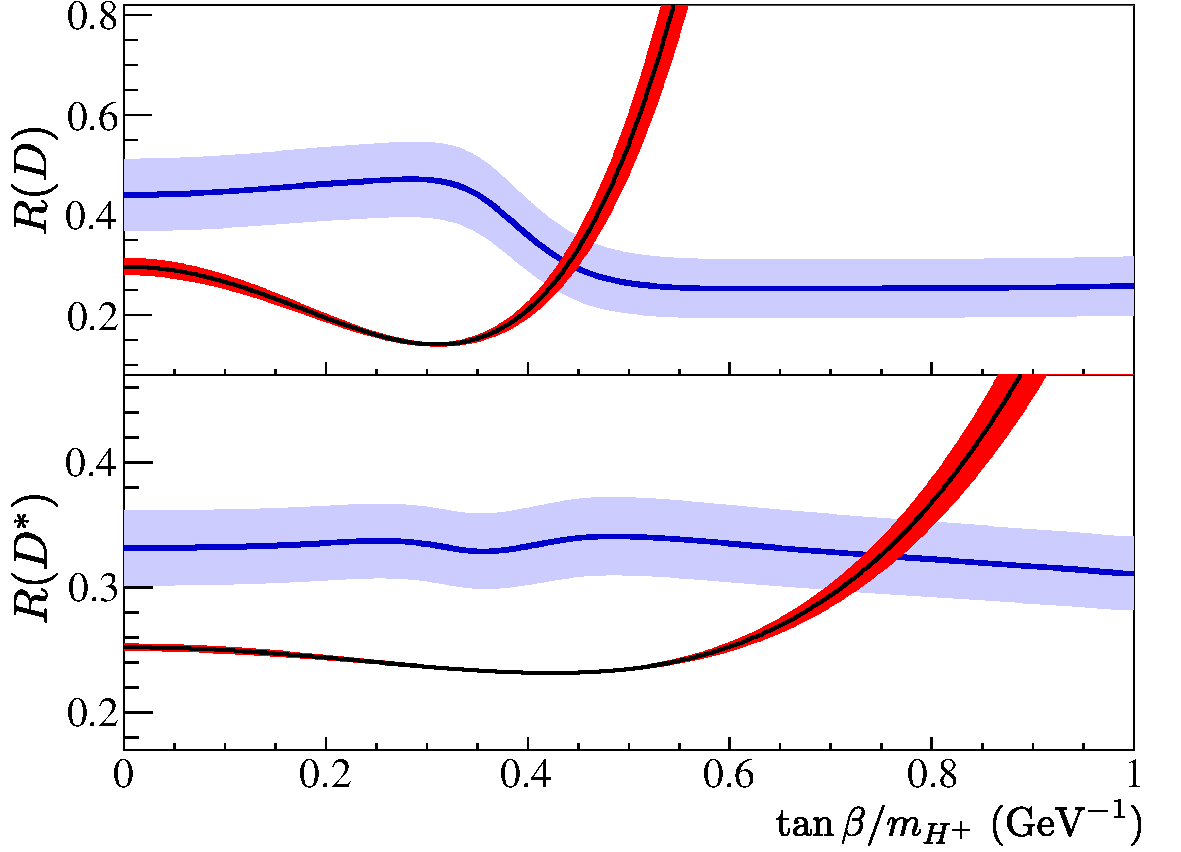
\includegraphics[width=8cm]{figures/type2_2hdm_vs_rd_rds_1205_5442.pdf}	
	}
	\only<2>{
		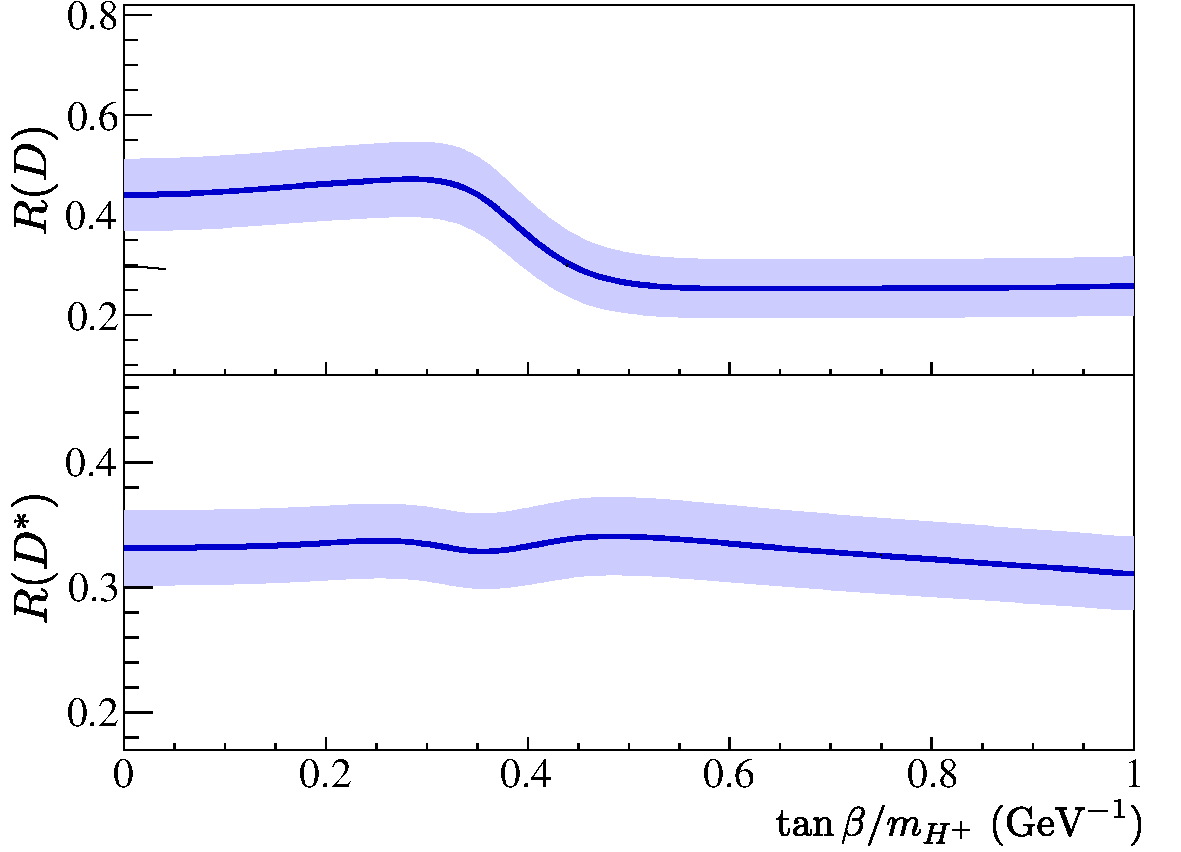
\includegraphics[width=8cm]{figures/type2_2hdm_vs_rd_rds_1205_5442_results_only.pdf}	
	}
	\end{center}
\end{frame}
%
%\begin{frame}{Clustering of $B\lra D^{(*)} l \nu$ kinematic shapes}
%	\textbf{Team:}
%	\begin{itemize}
%		\item Original idea/kickoff/implementation of distributions: \mauthor{Alejandro Celis} \\
%		(left in November 2018) 
%		\item Open development on \url{https://github.com/RD-clustering/B_decays_clustering/}
%		\item Also on board: \mauthor{Jason Aebischer}
%	\end{itemize}
%	\textbf{Problem:} Phenomenology of NP models depends on free parameters influencing the shape of kinematic distributions $\Lra$
%	\begin{itemize}
%		\item Difficult to present exclusion limits
%		\item An issue for analyses that need to make assumptions on kinematic distributions to extract features of interest (but still want to publish their results in a very general way)
%	\end{itemize}
%	\textbf{Solution:}
%	\begin{itemize}
%		\item Cluster NP parameter space based on a metric quantifying similarity of the result kinematic distributions
%		\item Choose NP benchmark point representing each cluster cluster
%		\item Report exclusion limits and measurements for each benchmark point
%	\end{itemize}
%\end{frame}
%%
%%
%\begin{frame}
%	\textbf{Examples:}
%	\begin{itemize}
%		\item For 2HDMs: \reference{https://arxiv.org/abs/1507.02245}{1507.02245} (used by \mauthor{ATLAS} and \mauthor{CMS})
%		\item Example of the dependency of result based on hypothesis (\mauthor{BaBar}):\\
%		
%		\medskip
%		{\centering
%			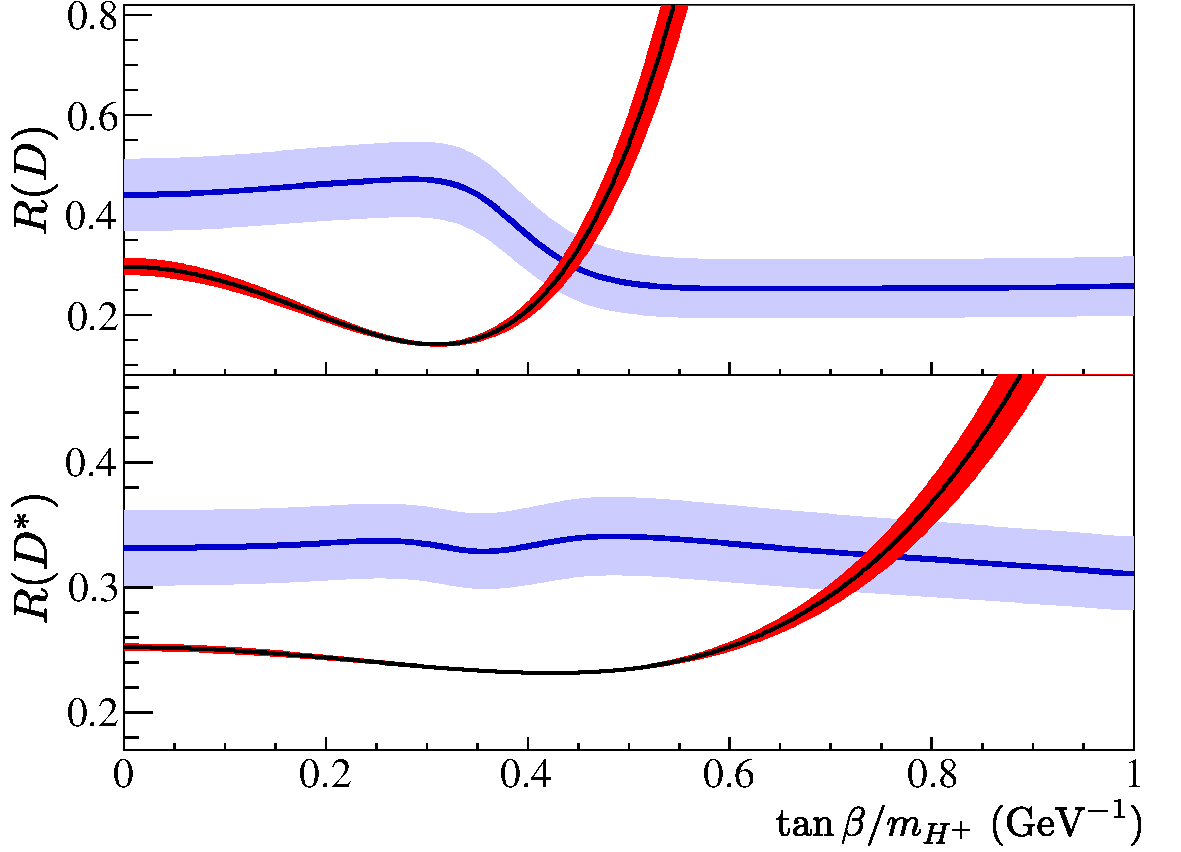
\includegraphics[width=8cm]{figures/type2_2hdm_vs_rd_rds_1205_5442.pdf}	
%			\par
%		}
%	\end{itemize}
%\end{frame}